% Options for packages loaded elsewhere
\PassOptionsToPackage{unicode}{hyperref}
\PassOptionsToPackage{hyphens}{url}
%
\documentclass[
  ignorenonframetext,
]{beamer}
\usepackage{pgfpages}
\setbeamertemplate{caption}[numbered]
\setbeamertemplate{caption label separator}{: }
\setbeamercolor{caption name}{fg=normal text.fg}
\beamertemplatenavigationsymbolsempty
% Prevent slide breaks in the middle of a paragraph
\widowpenalties 1 10000
\raggedbottom
\setbeamertemplate{part page}{
  \centering
  \begin{beamercolorbox}[sep=16pt,center]{part title}
    \usebeamerfont{part title}\insertpart\par
  \end{beamercolorbox}
}
\setbeamertemplate{section page}{
  \centering
  \begin{beamercolorbox}[sep=12pt,center]{part title}
    \usebeamerfont{section title}\insertsection\par
  \end{beamercolorbox}
}
\setbeamertemplate{subsection page}{
  \centering
  \begin{beamercolorbox}[sep=8pt,center]{part title}
    \usebeamerfont{subsection title}\insertsubsection\par
  \end{beamercolorbox}
}
\AtBeginPart{
  \frame{\partpage}
}
\AtBeginSection{
  \ifbibliography
  \else
    \frame{\sectionpage}
  \fi
}
\AtBeginSubsection{
  \frame{\subsectionpage}
}
\usepackage{amsmath,amssymb}
\usepackage{lmodern}
\usepackage{iftex}
\ifPDFTeX
  \usepackage[T1]{fontenc}
  \usepackage[utf8]{inputenc}
  \usepackage{textcomp} % provide euro and other symbols
\else % if luatex or xetex
  \usepackage{unicode-math}
  \defaultfontfeatures{Scale=MatchLowercase}
  \defaultfontfeatures[\rmfamily]{Ligatures=TeX,Scale=1}
\fi
% Use upquote if available, for straight quotes in verbatim environments
\IfFileExists{upquote.sty}{\usepackage{upquote}}{}
\IfFileExists{microtype.sty}{% use microtype if available
  \usepackage[]{microtype}
  \UseMicrotypeSet[protrusion]{basicmath} % disable protrusion for tt fonts
}{}
\makeatletter
\@ifundefined{KOMAClassName}{% if non-KOMA class
  \IfFileExists{parskip.sty}{%
    \usepackage{parskip}
  }{% else
    \setlength{\parindent}{0pt}
    \setlength{\parskip}{6pt plus 2pt minus 1pt}}
}{% if KOMA class
  \KOMAoptions{parskip=half}}
\makeatother
\usepackage{xcolor}
\IfFileExists{xurl.sty}{\usepackage{xurl}}{} % add URL line breaks if available
\IfFileExists{bookmark.sty}{\usepackage{bookmark}}{\usepackage{hyperref}}
\hypersetup{
  pdftitle={Logistic Regression: Case study},
  pdfauthor={Jyotishka Datta (jyotishka@vt.edu)   Department of Statistics, Virginia Tech},
  hidelinks,
  pdfcreator={LaTeX via pandoc}}
\urlstyle{same} % disable monospaced font for URLs
\newif\ifbibliography
\usepackage{color}
\usepackage{fancyvrb}
\newcommand{\VerbBar}{|}
\newcommand{\VERB}{\Verb[commandchars=\\\{\}]}
\DefineVerbatimEnvironment{Highlighting}{Verbatim}{commandchars=\\\{\}}
% Add ',fontsize=\small' for more characters per line
\usepackage{framed}
\definecolor{shadecolor}{RGB}{248,248,248}
\newenvironment{Shaded}{\begin{snugshade}}{\end{snugshade}}
\newcommand{\AlertTok}[1]{\textcolor[rgb]{0.94,0.16,0.16}{#1}}
\newcommand{\AnnotationTok}[1]{\textcolor[rgb]{0.56,0.35,0.01}{\textbf{\textit{#1}}}}
\newcommand{\AttributeTok}[1]{\textcolor[rgb]{0.77,0.63,0.00}{#1}}
\newcommand{\BaseNTok}[1]{\textcolor[rgb]{0.00,0.00,0.81}{#1}}
\newcommand{\BuiltInTok}[1]{#1}
\newcommand{\CharTok}[1]{\textcolor[rgb]{0.31,0.60,0.02}{#1}}
\newcommand{\CommentTok}[1]{\textcolor[rgb]{0.56,0.35,0.01}{\textit{#1}}}
\newcommand{\CommentVarTok}[1]{\textcolor[rgb]{0.56,0.35,0.01}{\textbf{\textit{#1}}}}
\newcommand{\ConstantTok}[1]{\textcolor[rgb]{0.00,0.00,0.00}{#1}}
\newcommand{\ControlFlowTok}[1]{\textcolor[rgb]{0.13,0.29,0.53}{\textbf{#1}}}
\newcommand{\DataTypeTok}[1]{\textcolor[rgb]{0.13,0.29,0.53}{#1}}
\newcommand{\DecValTok}[1]{\textcolor[rgb]{0.00,0.00,0.81}{#1}}
\newcommand{\DocumentationTok}[1]{\textcolor[rgb]{0.56,0.35,0.01}{\textbf{\textit{#1}}}}
\newcommand{\ErrorTok}[1]{\textcolor[rgb]{0.64,0.00,0.00}{\textbf{#1}}}
\newcommand{\ExtensionTok}[1]{#1}
\newcommand{\FloatTok}[1]{\textcolor[rgb]{0.00,0.00,0.81}{#1}}
\newcommand{\FunctionTok}[1]{\textcolor[rgb]{0.00,0.00,0.00}{#1}}
\newcommand{\ImportTok}[1]{#1}
\newcommand{\InformationTok}[1]{\textcolor[rgb]{0.56,0.35,0.01}{\textbf{\textit{#1}}}}
\newcommand{\KeywordTok}[1]{\textcolor[rgb]{0.13,0.29,0.53}{\textbf{#1}}}
\newcommand{\NormalTok}[1]{#1}
\newcommand{\OperatorTok}[1]{\textcolor[rgb]{0.81,0.36,0.00}{\textbf{#1}}}
\newcommand{\OtherTok}[1]{\textcolor[rgb]{0.56,0.35,0.01}{#1}}
\newcommand{\PreprocessorTok}[1]{\textcolor[rgb]{0.56,0.35,0.01}{\textit{#1}}}
\newcommand{\RegionMarkerTok}[1]{#1}
\newcommand{\SpecialCharTok}[1]{\textcolor[rgb]{0.00,0.00,0.00}{#1}}
\newcommand{\SpecialStringTok}[1]{\textcolor[rgb]{0.31,0.60,0.02}{#1}}
\newcommand{\StringTok}[1]{\textcolor[rgb]{0.31,0.60,0.02}{#1}}
\newcommand{\VariableTok}[1]{\textcolor[rgb]{0.00,0.00,0.00}{#1}}
\newcommand{\VerbatimStringTok}[1]{\textcolor[rgb]{0.31,0.60,0.02}{#1}}
\newcommand{\WarningTok}[1]{\textcolor[rgb]{0.56,0.35,0.01}{\textbf{\textit{#1}}}}
\usepackage{graphicx}
\makeatletter
\def\maxwidth{\ifdim\Gin@nat@width>\linewidth\linewidth\else\Gin@nat@width\fi}
\def\maxheight{\ifdim\Gin@nat@height>\textheight\textheight\else\Gin@nat@height\fi}
\makeatother
% Scale images if necessary, so that they will not overflow the page
% margins by default, and it is still possible to overwrite the defaults
% using explicit options in \includegraphics[width, height, ...]{}
\setkeys{Gin}{width=\maxwidth,height=\maxheight,keepaspectratio}
% Set default figure placement to htbp
\makeatletter
\def\fps@figure{htbp}
\makeatother
\setlength{\emergencystretch}{3em} % prevent overfull lines
\providecommand{\tightlist}{%
  \setlength{\itemsep}{0pt}\setlength{\parskip}{0pt}}
\setcounter{secnumdepth}{-\maxdimen} % remove section numbering
\ifLuaTeX
  \usepackage{selnolig}  % disable illegal ligatures
\fi

\title{Logistic Regression: Case study}
\author{Jyotishka Datta
(\href{mailto:jyotishka@vt.edu}{\nolinkurl{jyotishka@vt.edu}})
Department of Statistics, Virginia Tech}
\date{2022-03-17}

\begin{document}
\frame{\titlepage}

\begin{frame}{Challenger case study}
\protect\hypertarget{challenger-case-study}{}
\begin{itemize}
\item
  Today we will look at an (in)famous example of applying regression to
  data where assumptions were not met and failure to account for
  modeling errors led to a huge disaster.
\item
  This example is taken from ``Statistics for Social Sciences II:
  Multivariate Techniques'' by Eduardo García Portugués.
\end{itemize}
\end{frame}

\begin{frame}{Challenger}
\protect\hypertarget{challenger}{}
\begin{itemize}
\item
  On January 28, 1986 NASA Space Shuttle orbiter Challenger broke apart
  and disintegrated at 73 seconds into its flight, leading to the deaths
  of its seven crew members.
\item
  Had serious consequences for credibility and mass perception
\item
  The Presidential Rogers Commission (formed by astronaut Neil A.
  Armstrong and Nobel laureate Richard P. Feynman, among others) was
  created to investigate the disaster.
\item
  The commission determined that the disintegration began with the
  failure of an O-ring seal in the solid rocket motor due to the unusual
  cold temperatures (-0.6 Celsius degrees) during the launch.
\end{itemize}
\end{frame}

\begin{frame}{O-rings}
\protect\hypertarget{o-rings}{}
\begin{itemize}
\tightlist
\item
  \textbf{The problematic with O-rings was something known:} the night
  before the launch, there was a three-hour teleconference between motor
  engineers and NASA management, discussing the effect of low
  temperature forecasted for the launch on the O-ring performance. The
  conclusion, influenced by Figure 4.2a, was:
\end{itemize}

\begin{quote}
``Temperature data {[}are{]} not conclusive on predicting primary O-ring
blowby.''
\end{quote}
\end{frame}

\begin{frame}{Figure from the report}
\protect\hypertarget{figure-from-the-report}{}
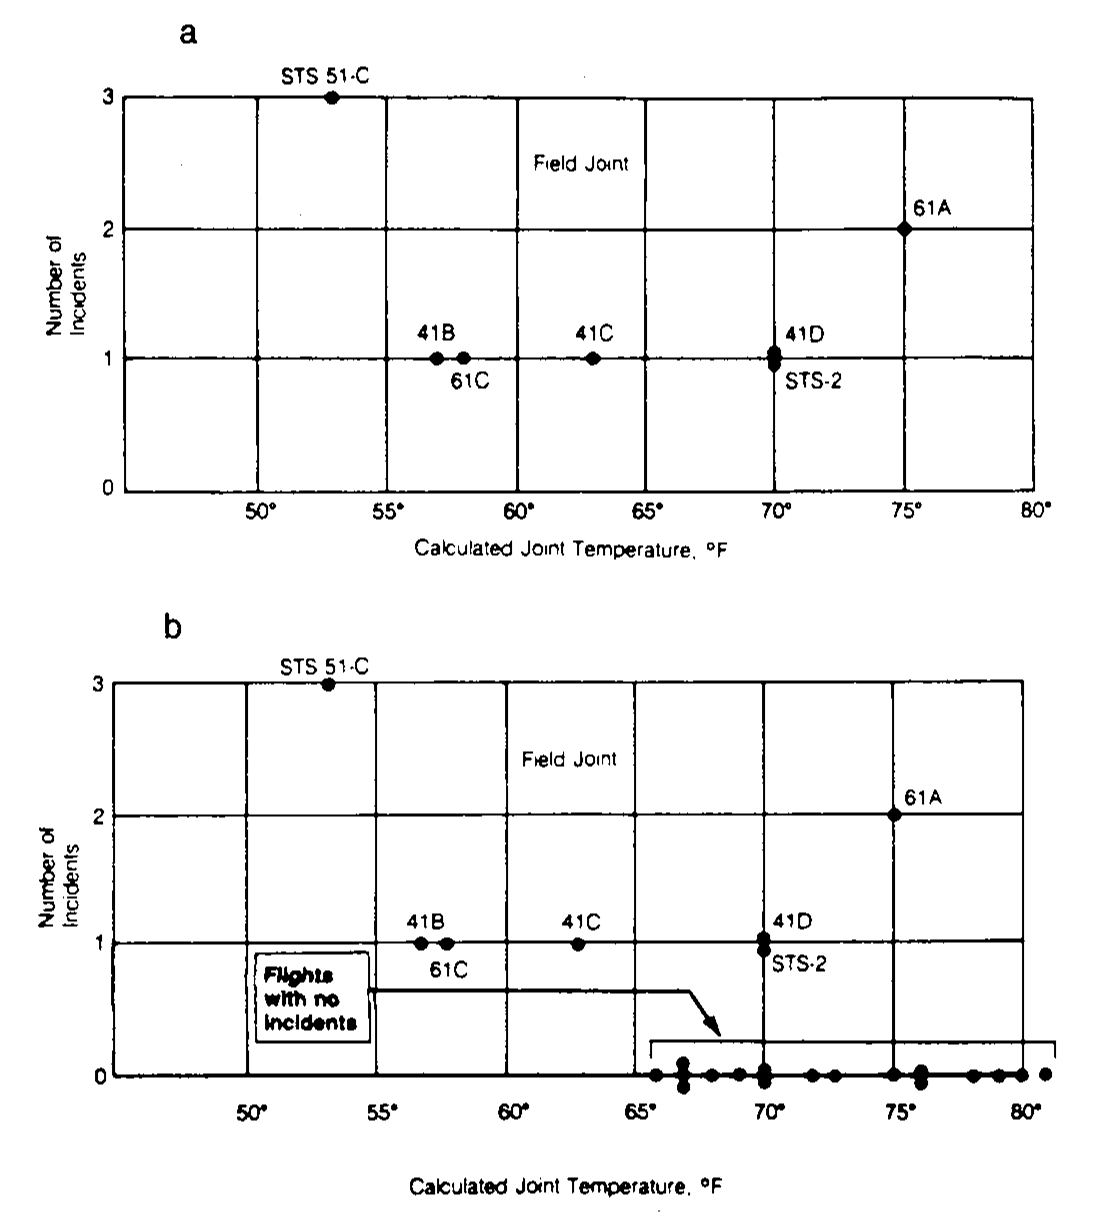
\includegraphics[width=0.5\textwidth,height=\textheight]{challenger.png}
\end{frame}

\begin{frame}{Rogers commission}
\protect\hypertarget{rogers-commission}{}
\begin{itemize}
\tightlist
\item
  Rogers Commission noted a major flaw in this Figure :
\end{itemize}

\begin{quote}
``the flights with zero incidents were excluded from the plot because it
was felt that these flights did not contribute any information about the
temperature effect.''
\end{quote}

The Rogers Commission concluded:

``A careful analysis of the flight history of O-ring performance would
have revealed the correlation of O-ring damage in low temperature''.
\end{frame}

\begin{frame}{Dalal, Fowlkes, and Hoadley (1989)}
\protect\hypertarget{dalal-fowlkes-and-hoadley-1989}{}
\begin{itemize}
\tightlist
\item
  Q1. Is the temperature associated with O-ring incidents?
\item
  Q2. In which way was the temperature affecting the probability of
  O-ring incidents?
\item
  Q3. What was the predicted probability of an incident in an O-ring for
  the temperature of the launch day?
\end{itemize}
\end{frame}

\begin{frame}[fragile]{Data-set}
\protect\hypertarget{data-set}{}
\begin{verbatim}
## 'data.frame':    23 obs. of  9 variables:
##  $ flight       : chr  "1" "2" "3" "5" ...
##  $ date         : chr  "12/04/81" "12/11/81" "22/03/82" "11/11/82" ...
##  $ nfails.field : int  0 1 0 0 0 0 0 0 1 1 ...
##  $ nfails.nozzle: int  0 0 0 0 2 0 0 0 1 1 ...
##  $ fail.field   : int  0 1 0 0 0 0 0 0 1 1 ...
##  $ fail.nozzle  : int  0 0 0 0 1 0 0 0 1 1 ...
##  $ temp         : num  18.9 21.1 20.6 20 19.4 22.2 22.8 21.1 13.9 17.2 ...
##  $ pres.field   : int  50 50 50 50 50 50 100 100 100 200 ...
##  $ pres.nozzle  : int  50 50 50 50 50 50 50 100 100 200 ...
\end{verbatim}
\end{frame}

\begin{frame}[fragile]{Important variables}
\protect\hypertarget{important-variables}{}
\begin{itemize}
\item
  \texttt{fail.field}, \texttt{fail.nozzle}: binary variables indicating
  whether there was an incident with the O-rings in the field joints or
  in the nozzles of the solid rocket boosters. 1 codifies an incident
  and 0 its absence. On the analysis, we focus on the O-rings of the
  field joint as being the most determinants for the accident.
  (\texttt{nfails.field}, \texttt{nfails.nozzle}: total numbers.)
\item
  \texttt{temp}: temperature in the day of launch. Measured in Celsius
  degrees.
\item
  \texttt{pres.field}, \texttt{pres.nozzle}: leak-check pressure tests
  of the O-rings. These tests assured that the rings would seal the
  joint.
\end{itemize}
\end{frame}

\begin{frame}[fragile]{Try to recreate}
\protect\hypertarget{try-to-recreate}{}
\begin{itemize}
\item
  We make two scatterplots of \texttt{nfails.field} (number of total
  incidents in the field joints) versus temp,
\item
  The first one excluding the launches without incidents (subset =
  \texttt{nfails.field\ \textgreater{}\ 0}) and the second one for all
  the data.
\end{itemize}
\end{frame}

\begin{frame}{Without incidents}
\protect\hypertarget{without-incidents}{}
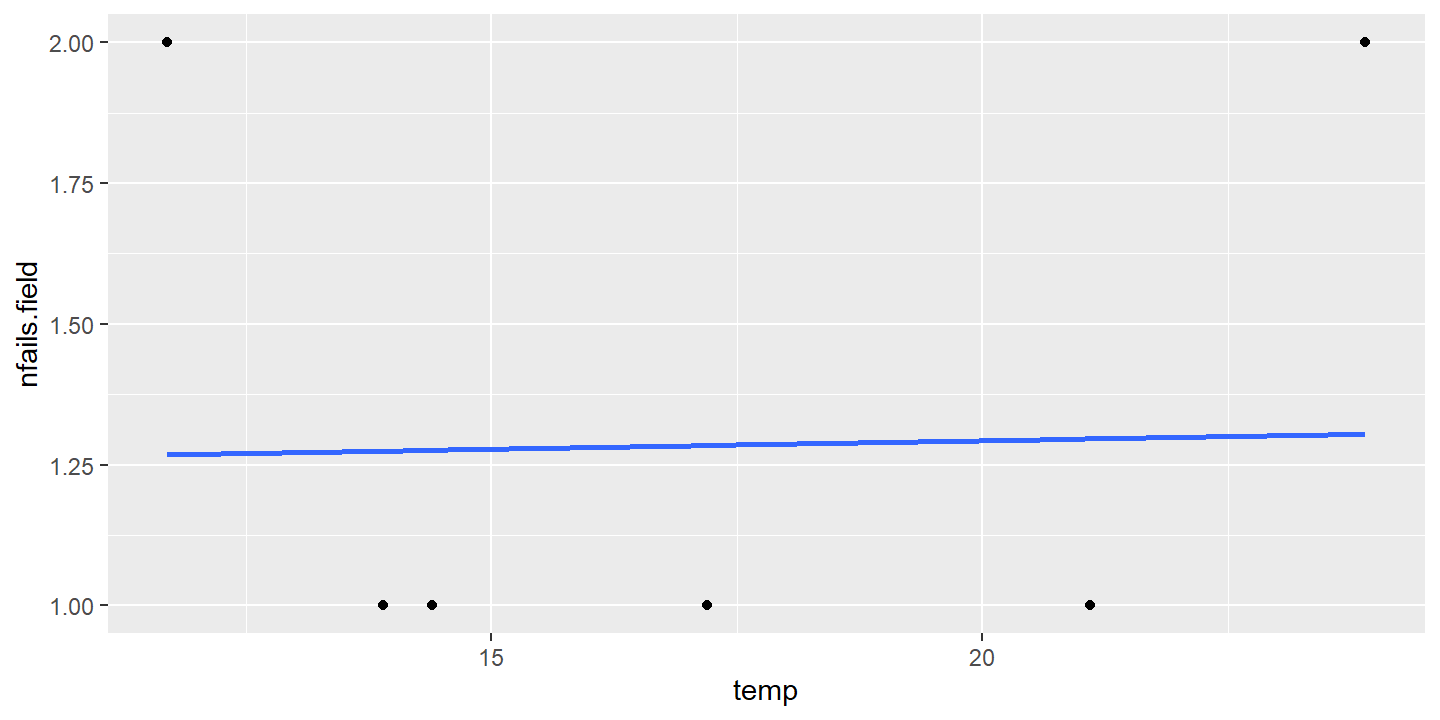
\includegraphics{logistic_challenger_files/figure-beamer/scatter1-1.pdf}
\end{frame}

\begin{frame}{With incidents}
\protect\hypertarget{with-incidents}{}
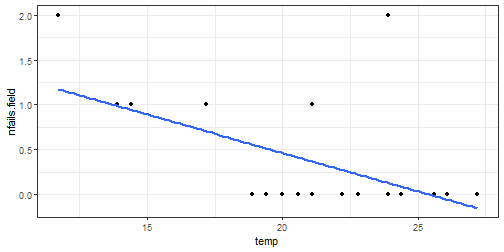
\includegraphics{logistic_challenger_files/figure-beamer/scatter2-1.pdf}
\end{frame}

\begin{frame}{Major problems}
\protect\hypertarget{major-problems}{}
\begin{itemize}
\item
  There is a fundamental problem in using linear regression for this
  data: \textbf{the response is not continuous}.
\item
  As a consequence, there is no linearity and the errors around the mean
  are not normal (indeed, they are strongly non normal).
\item
  Recall LM assumption:
  \([ y \mid x] \sim N(\beta_0 + \beta_1 x, \sigma^2)\)
\end{itemize}
\end{frame}

\begin{frame}{How do we check}
\protect\hypertarget{how-do-we-check}{}
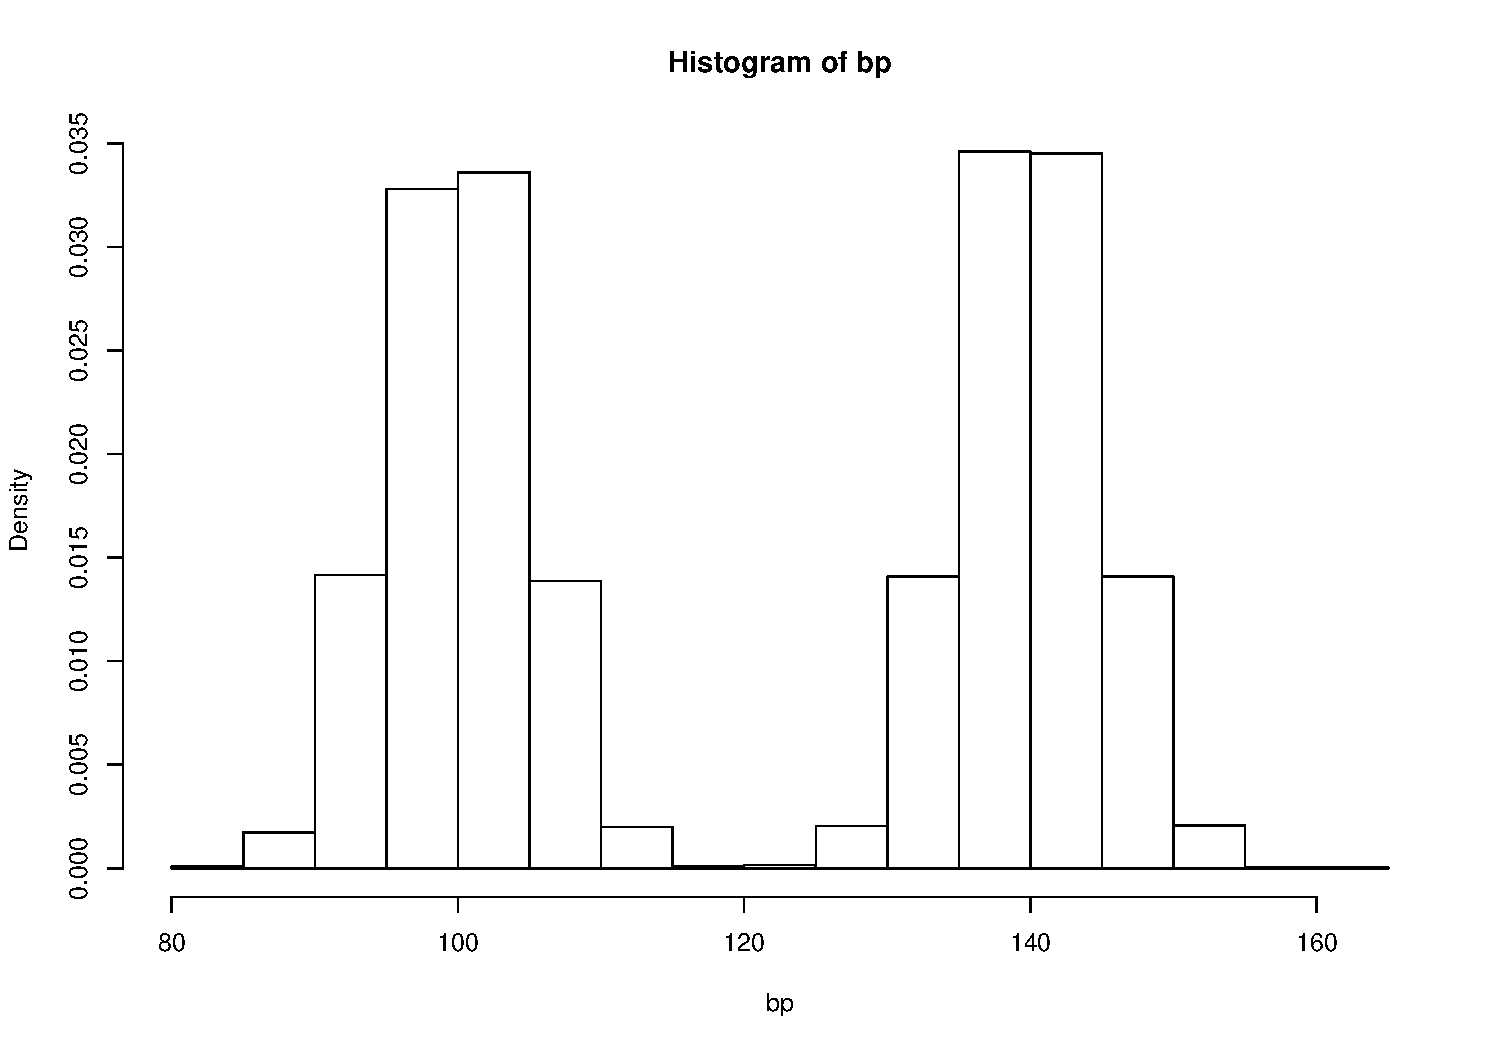
\includegraphics{logistic_challenger_files/figure-beamer/unnamed-chunk-2-1.pdf}
\end{frame}

\hypertarget{logistic}{%
\section{Logistic}\label{logistic}}

\begin{frame}[fragile]{Recall}
\protect\hypertarget{recall}{}
\begin{itemize}
\item
  Instead of modeling the number of incidents which is definitely not
  normal, we will take a different approach: We'll model the probability
  of expecting at least one incident given the temperature: \[
  p(x) = \mathbb{P}(\text{incident} = 1 | \text{temperature} = x)
  \]
\item
  These two will come from \texttt{fail.field} and \texttt{temp}
\item
  The logistic model would be: \[
  p(x) = \text{logistic}(\beta_0 + \beta_1x) = \frac{e^{\beta_0 + \beta_1x}}{1 + e^{\beta_0 + \beta_1x}}
  \]
\end{itemize}
\end{frame}

\begin{frame}[fragile]{Logistic Regression}
\protect\hypertarget{logistic-regression}{}
We will use R to fit a logistic regression model in order to predict
\texttt{fali.field} using \texttt{temp}.

The \texttt{glm()} function fits generalized linear models, a class of
models that includes logistic regression.

The syntax of the \texttt{glm()} function is similar to that of
\texttt{lm()}, except that we must pass in linear model the argument
\texttt{family=binomial} in order to tell \texttt{R} to run a logistic
regression rather than some other type of generalized linear model.
\end{frame}

\begin{frame}[fragile]{Output}
\protect\hypertarget{output}{}
\begin{verbatim}
## 
## Call:
## glm(formula = fail.field ~ temp, family = "binomial", data = challenger)
## 
## Deviance Residuals: 
##     Min       1Q   Median       3Q      Max  
## -1.0566  -0.7575  -0.3818   0.4571   2.2195  
## 
## Coefficients:
##             Estimate Std. Error z value Pr(>|z|)  
## (Intercept)   7.5837     3.9146   1.937   0.0527 .
## temp         -0.4166     0.1940  -2.147   0.0318 *
## ---
## Signif. codes:  0 '***' 0.001 '**' 0.01 '*' 0.05 '.' 0.1 ' ' 1
## 
## (Dispersion parameter for binomial family taken to be 1)
## 
##     Null deviance: 28.267  on 22  degrees of freedom
## Residual deviance: 20.335  on 21  degrees of freedom
## AIC: 24.335
## 
## Number of Fisher Scoring iterations: 5
\end{verbatim}
\end{frame}

\begin{frame}{Interpretation}
\protect\hypertarget{interpretation}{}
The summary of the logistic model is notably different from the linear
regression, as the methodology behind is quite different.

Nevertheless, we have tests for the significance of each coefficient.

Here we obtain that temp is significantly different from zero, at least
at a level \(\alpha = 0.05\).

Therefore we can conclude that the temperature is indeed affecting the
probability of an incident with the O-rings.
\end{frame}

\begin{frame}[fragile]{Coefficients}
\protect\hypertarget{coefficients}{}
\begin{itemize}
\item
  To interpret the coefficients, we have to be careful.
\item
  Here our model is: \[
  \text{logit}(P(\text{incident} = 1 | \text{temp} = x) = \beta_0 + \beta_1 x \\
  \text{where } \text{logit}(p) = \frac{p}{1-p}
  \]
\end{itemize}

\begin{verbatim}
##  (Intercept)         temp 
## 1965.9743592    0.6592539
\end{verbatim}
\end{frame}

\begin{frame}[fragile]{We will draw the curve}
\protect\hypertarget{we-will-draw-the-curve}{}
\begin{itemize}
\item
  We are going to plot the logistic sigmoid for a grid of \(x\),
  i.e.~temparature values.
\item
  Recall \(\text{logistic}(x) = 1/(1 + e^{-x})\).
\item
  We are plotting \(\text{logistic}(\hat{\beta}_0 + \hat{\beta}_1 x)\),
  with \(\hat{\beta}_0\) and \(\hat{\beta}_1\) from glm output.
\end{itemize}

\begin{Shaded}
\begin{Highlighting}[]
\CommentTok{\# Plot data}
\FunctionTok{plot}\NormalTok{(challenger}\SpecialCharTok{$}\NormalTok{temp, challenger}\SpecialCharTok{$}\NormalTok{fail.field, }\AttributeTok{xlim =} \FunctionTok{c}\NormalTok{(}\SpecialCharTok{{-}}\DecValTok{1}\NormalTok{, }\DecValTok{30}\NormalTok{), }\AttributeTok{xlab =} \StringTok{"Temperature"}\NormalTok{,}
     \AttributeTok{ylab =} \StringTok{"Incident probability"}\NormalTok{)}

\CommentTok{\# Draw the fitted logistic curve}
\NormalTok{x }\OtherTok{\textless{}{-}} \FunctionTok{seq}\NormalTok{(}\SpecialCharTok{{-}}\DecValTok{1}\NormalTok{, }\DecValTok{30}\NormalTok{, }\AttributeTok{l =} \DecValTok{200}\NormalTok{)}
\NormalTok{y }\OtherTok{\textless{}{-}} \FunctionTok{exp}\NormalTok{(}\SpecialCharTok{{-}}\NormalTok{(nasa}\SpecialCharTok{$}\NormalTok{coefficients[}\DecValTok{1}\NormalTok{] }\SpecialCharTok{+}\NormalTok{ nasa}\SpecialCharTok{$}\NormalTok{coefficients[}\DecValTok{2}\NormalTok{] }\SpecialCharTok{*}\NormalTok{ x))}
\NormalTok{y }\OtherTok{\textless{}{-}} \DecValTok{1} \SpecialCharTok{/}\NormalTok{ (}\DecValTok{1} \SpecialCharTok{+}\NormalTok{ y)}
\FunctionTok{lines}\NormalTok{(x, y, }\AttributeTok{col =} \DecValTok{2}\NormalTok{, }\AttributeTok{lwd =} \DecValTok{2}\NormalTok{)}
\end{Highlighting}
\end{Shaded}
\end{frame}

\begin{frame}{We will draw the curve}
\protect\hypertarget{we-will-draw-the-curve-1}{}
At the sight of this curve and the summary of the model we can conclude
that the temperature was increasing the probability of an O-ring
incident (Q2).

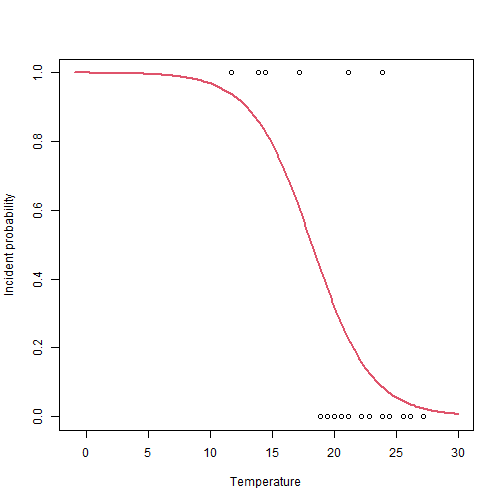
\includegraphics{logistic_challenger_files/figure-beamer/logistic_curve2-1.pdf}
\end{frame}

\begin{frame}{Add challenger to it}
\protect\hypertarget{add-challenger-to-it}{}
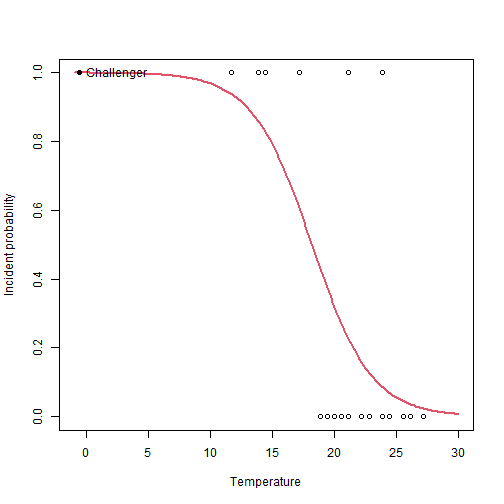
\includegraphics{logistic_challenger_files/figure-beamer/logistic_curve3-1.pdf}
\end{frame}

\begin{frame}[fragile]{Prediction}
\protect\hypertarget{prediction}{}
Finally, the probability of having at least one incident with the
O-rings in the launch day was 0.9996 according to the fitted logistic
model (Q3). This is easily obtained:

\begin{verbatim}
##        1 
## 0.999604
\end{verbatim}

Be careful about extrapolations, though!
\end{frame}

\end{document}
